\documentclass{article}
\usepackage{fullpage}
\usepackage{amsmath}
\usepackage{amsfonts}
\usepackage{tipa}
\usepackage{tikz}
\usepackage{gb4e}
\noautomath
\title{QP2 Topics}
\begin{document}
\maketitle
\section{Topics, Broadly Speaking}
For this QP, I'm considering (at least) two broad topics: checked tone in Chinese dialects, and tone sandhi alternations.
\begin{itemize}
	\item Checked Tone
	\begin{itemize}
		\item How to represent it?
		\item In terms of local restrictions?
		\item In terms of melody restrictions?
		\item As an $I \rightarrow O$ process?
		\item Can its representation tell us about its learnability?
	\end{itemize}
	\item Tone Sandhi
	\begin{itemize}
		\item How to formalize the notion that tone sandhi is an inherently \textit{prosodic} phenomenon?
		\item Sandhi happens within a domain; span? foot?
		\item Directional asymmetries (right-dominant, left-dominant), are they due to prominence or stress?
		\item How are tone sandhi processes learned?
		\item Take a step back from a particular formalism (OT, representation)
	\end{itemize}
\end{itemize}
The interest in checked tone comes from a problem I started working on in my MA thesis, which looked at the representation of checked tone in the Nanjing dialect.
\section{Nanjing Checked Tone and a (Possible) Subset Problem}
The following tonal structures are illformed in the Nanjing dialect. This assumes that checked tone is monomoraic, with a single mora attaching to a H segment.
\newpage
\begin{exe}
\ex \
\begin{center}
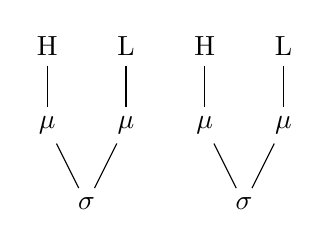
\begin{tikzpicture}
	\node (H1) at (-2,1){H};
	\node (L1) at (-1,1) {L};
	\node (H2) at (0,1){H};
	\node (L2) at (1,1) {L};
	\node (m1) at (-2,0){$\mu$};
	\node (m2) at (-1,0) {$\mu$};
	\node (m3) at (0,0){$\mu$};
	\node (m4) at (1,0) {$\mu$};
	\node (s1) at (-1.5, -1) {$\sigma$};
	\node (s2) at (.5, -1) {$\sigma$};
	\draw [-] (H1) -- (m1);
	\draw [-] (L1) -- (m2);
	\draw [-] (H2) -- (m3);
	\draw [-] (L2) -- (m4);
	\draw [-] (m1) -- (s1);
	\draw [-] (m2) -- (s1);
	\draw [-] (m3) -- (s2);
	\draw [-] (m4) -- (s2);
\end{tikzpicture}
\hspace{2cm}
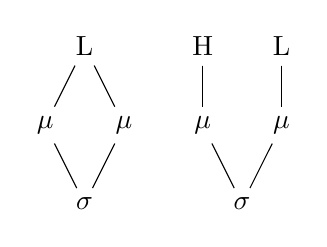
\begin{tikzpicture}
	\node (H1) at (-1.5,1){L};
	\node (H2) at (0,1){H};
	\node (L2) at (1,1) {L};
	\node (m1) at (-2,0){$\mu$};
	\node (m2) at (-1,0) {$\mu$};
	\node (m3) at (0,0){$\mu$};
	\node (m4) at (1,0) {$\mu$};
	\node (s1) at (-1.5, -1) {$\sigma$};
	\node (s2) at (.5, -1) {$\sigma$};
	\draw [-] (H1) -- (m1);
	\draw [-] (H1) -- (m2);
	\draw [-] (H2) -- (m3);
	\draw [-] (L2) -- (m4);
	\draw [-] (H2) -- (m3);
	\draw [-] (L2) -- (m4);
	\draw [-] (m1) -- (s1);
	\draw [-] (m2) -- (s1);
	\draw [-] (m3) -- (s2);
	\draw [-] (m4) -- (s2);
\end{tikzpicture}
\hspace{2cm}
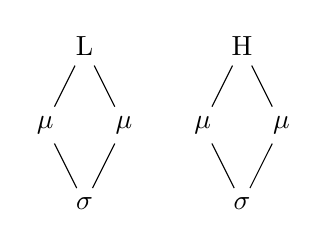
\begin{tikzpicture}
	\node (L1) at (-1.5,1){L};
	\node (H1) at (0.5,1){H};
	\node (m1) at (-2,0){$\mu$};
	\node (m2) at (-1,0) {$\mu$};
	\node (m3) at (0,0){$\mu$};
	\node (m4) at (1,0) {$\mu$};
	\node (s1) at (-1.5, -1) {$\sigma$};
	\node (s2) at (.5, -1) {$\sigma$};
	\draw [-] (L1) -- (m1);
	\draw [-] (L1) -- (m2);
	\draw [-] (H1) -- (m3);
	\draw [-] (H1) -- (m4);
	\draw [-] (m1) -- (s1);
	\draw [-] (m2) -- (s1);
	\draw [-] (m3) -- (s2);
	\draw [-] (m4) -- (s2);
\end{tikzpicture}\\
\vspace{2cm}
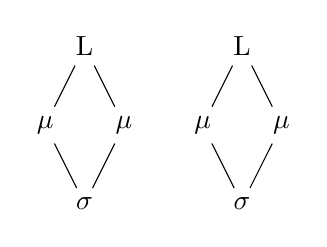
\begin{tikzpicture}
	\node (L1) at (-1.5,1){L};
	\node (H1) at (0.5,1){L};
	\node (m1) at (-2,0){$\mu$};
	\node (m2) at (-1,0) {$\mu$};
	\node (m3) at (0,0){$\mu$};
	\node (m4) at (1,0) {$\mu$};
	\node (s1) at (-1.5, -1) {$\sigma$};
	\node (s2) at (.5, -1) {$\sigma$};
	\draw [-] (L1) -- (m1);
	\draw [-] (L1) -- (m2);
	\draw [-] (H1) -- (m3);
	\draw [-] (H1) -- (m4);
	\draw [-] (m1) -- (s1);
	\draw [-] (m2) -- (s1);
	\draw [-] (m3) -- (s2);
	\draw [-] (m4) -- (s2);
\end{tikzpicture}
\hspace{2.1cm}
\begin{tikzpicture}
	\node (L1) at (-2,1){L};
	\node (H1) at (-1,1) {H};
	\node (H3) at (0.5,1){H};
	\node (m1) at (-2,0){$\mu$};
	\node (m2) at (-1,0) {$\mu$};
	\node (m3) at (.5,0){$\mu$};
	\node (s1) at (-1.5, -1) {$\sigma$};
	\node (s2) at (.5, -1) {$\sigma$};
	\draw [-] (L1) -- (m1);
	\draw [-] (H1) -- (m2);
	\draw [-] (H3) -- (m3);
	\draw [-] (m1) -- (s1);
	\draw [-] (m2) -- (s1);
	\draw [-] (m3) -- (s2);
\end{tikzpicture}
\hspace{2.1cm}
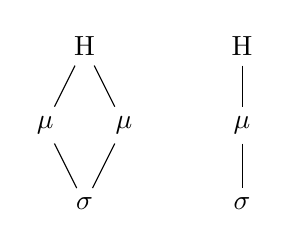
\begin{tikzpicture}
	\node (H1) at (-1.5,1){H};
	\node (H2) at (0.5,1){H};
	\node (m1) at (-2,0){$\mu$};
	\node (m2) at (-1,0) {$\mu$};
	\node (m3) at (.5,0){$\mu$};
	\node (s1) at (-1.5, -1) {$\sigma$};
	\node (s2) at (.5, -1) {$\sigma$};
	\draw [-] (H1) -- (m1);
	\draw [-] (H1) -- (m2);
	\draw [-] (H2) -- (m3);
	\draw [-] (m1) -- (s1);
	\draw [-] (m2) -- (s1);
	\draw [-] (m3) -- (s2);
\end{tikzpicture}
\end{center}
\medskip{}
\end{exe}
The set of illicit substrings in the language is summarized in (2).
\begin{exe}
\ex $S_{NJ}$ = \{HLHL, LLHL, LLHH, LLLL, LHH, HHH\}
\end{exe}

There are a number of issues with this characterization. Primarily, there are licit forms in the language which contain members of $S_{NJ}$ as substrings, such as LHHH, and HHHH.
\begin{exe}
\ex \
\begin{center}
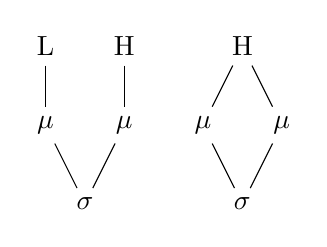
\begin{tikzpicture}
	\node (L1) at (-2,1){L};
	\node (H1) at (-1,1){H};
	\node (H2) at (.5,1) {H};
	\node (m1) at (-2,0){$\mu$};
	\node (m2) at (-1,0) {$\mu$};
	\node (m3) at (0,0){$\mu$};
	\node (m4) at (1,0) {$\mu$};
	\node (s1) at (-1.5, -1) {$\sigma$};
	\node (s2) at (.5, -1) {$\sigma$};
	\draw [-] (L1) -- (m1);
	\draw [-] (H1) -- (m2);
	\draw [-] (H2) -- (m3);
	\draw [-] (H2) -- (m4);
	\draw [-] (m1) -- (s1);
	\draw [-] (m2) -- (s1);
	\draw [-] (m3) -- (s2);
	\draw [-] (m4) -- (s2);
\end{tikzpicture}
\hspace{2cm}
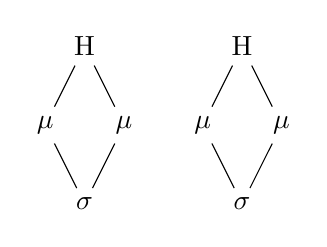
\begin{tikzpicture}
	\node (L1) at (-1.5,1){H};
	\node (H1) at (0.5,1){H};
	\node (m1) at (-2,0){$\mu$};
	\node (m2) at (-1,0) {$\mu$};
	\node (m3) at (0,0){$\mu$};
	\node (m4) at (1,0) {$\mu$};
	\node (s1) at (-1.5, -1) {$\sigma$};
	\node (s2) at (.5, -1) {$\sigma$};
	\draw [-] (L1) -- (m1);
	\draw [-] (L1) -- (m2);
	\draw [-] (H1) -- (m3);
	\draw [-] (H1) -- (m4);
	\draw [-] (m1) -- (s1);
	\draw [-] (m2) -- (s1);
	\draw [-] (m3) -- (s2);
	\draw [-] (m4) -- (s2);
\end{tikzpicture}
\end{center}
\end{exe}
Enriching the representation to include syllable boundaries (ex. *LH.H or *HH.H) or word boundaries (*LHH\# or *HHH\#) independently is of no help. Combining the two (*LH.H\# or *HH.H\#) does mitigate this issue. There is, however, a sense that what is at the heart of the issue is that a monomoraic [H]-toned syllable is different from a bimoraic one (as evidenced by the different sandhi patterns observed for each). Across dialects of Chinese, checked tones are defined not by a particular tonal representation, but by the presence of an obstruent (and sometimes sonorant, non-nasal) coda. The question is how to represent this distinction in a formal theory of tone sandhi. Segmental information cannot be encoded directly on the melodic tier, or in a string representation with tone-to-TBU associations. 

In my thesis, I capitalized on the notion of domains and local conjunction to isolate the sandhi environment which included checked-tone, but excluded bimoraic [H] syllables:
\begin{exe}
\ex *[HH, H\textipa{P}]$_{[H]}$: Assign one violation  to an H-element that occupies both HH and H\textipa{P} melodies
\end{exe}
Here, the domain of application is a single H-element. An unattractive component of this analysis is that it assumes [\textipa{P}] to be visible on the melodic tier, which is rather unconventional, and probably wrong.
\end{document}